\section{Szenario}

\subsection{Client/Server Anmeldungssystem}

\begin{frame}[c]

	\frametitle{Szenario}

	Ein \textbf{Client} möchte von einem \textbf{Server} Daten erhalten. 
	Hierzu muss der Client sich zunächst \textbf{autorisieren}.
	Erfolgreich autorisiert erhält der Client ein \textbf{Session-Schlüssel} 
	mit dem die darauf folgende Kommunikation verschlüsselt werden soll.
	Die vollständige Übertragung soll so ablaufen, 
	dass ein MITMA \textbf{weder} in der Lage sein soll, 
	zu erfahren wie das Passwort, der Benutzername 
	des Clients lauten \textbf{noch} soll der MITMA in der Lage 
	sein die Daten mitzulesen. Server und Client kennen hierzu, 
	genau so wie der MITMA, mindestens die öffentlichen Schlüssel von Server und Client.

\end{frame}

\subsection{Mögliche Realisierung}

\begin{frame}[c]
  \vfill
  \centering
  \begin{beamercolorbox}[sep=6pt,center,shadow=true,rounded=true]{title}
    \usebeamerfont{title}\textbf{\Large{\insertsubsectionhead}}\par%
  \end{beamercolorbox}
  \vfill
\end{frame}

\begin{frame}[t]

	\frametitle{Sequenz-Diagramm}

	\begin{center}
		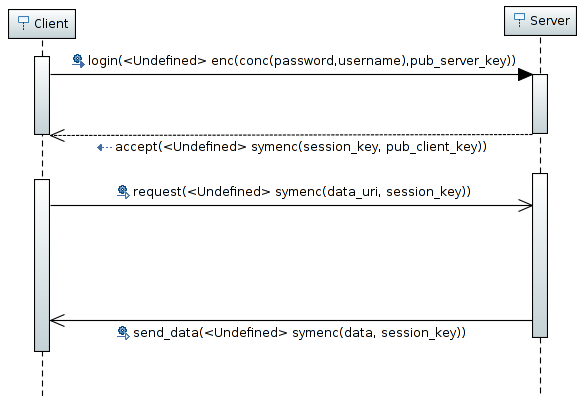
\includegraphics[width=220pt,angle=0]{../images/unsecure_seqdia.png}
	\end{center}
	
	\only<1-2>{
		%\begin{center}
			Dieses mittels Papyrus erstellte UML Sequenz-Diagramm könnte das besagte Szenario realisieren. 
			\textbf{Frage:} Ist diese Realisierung sicher?
			
			\vspace{0pt}
		%\end{center}
	}
	\only<2>{
		%\begin{center}
			Um dies zu überprüfen konfigurieren wir im folgenden das Plugin, lassen es das Diagramm analysieren 
			und beleuchten die dabei entstandene Analyse.
		%\end{center}
	}
	
%	Zunächst soll dieses mit Papyrus erstellte UML Sequenz-Diagramm das besagte Szenario realisieren. 
%	Im Folgenden Konfigurieren und erklären wir das Plugin und lassen es dann dieses Diagramm analysieren, 
%	um letztlich die Analyse näher zu beleuchten.

\end{frame}

\begin{frame}[t]

	\frametitle{Plugin Konfiguration}

	\begin{figure}[T]
		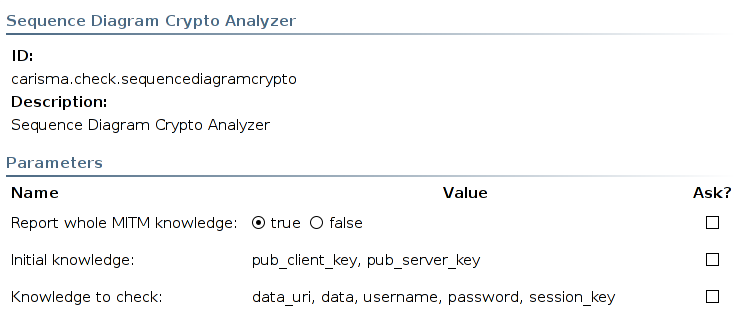
\includegraphics[width=290pt,angle=0]{../images/plugin_cfg.png}
	\end{figure}
	
	
	\only<1>{
		\begin{block}{Parameter}
			Das Plugin besitzt 3 Parameter: \textbf{Report whole MITM knowledge}, \textbf{Initial knowledge}
			und \textbf{Knowledge to check}.
		\end{block}
	}
	\only<2>{
		\begin{block}{Report whole MITM knowledge}
			Diese Einstellung ermöglicht es, das vollständige zur Überprüfung 
			notwendige MITM Wissen ausgeben zu lassen; Also das Wissen welches der potenzielle 
			MITMA erlangt zzgl. des Wissens welches zur Analyse der Sicherheit des Modells notwendig ist. 
		\end{block}
	}
	\only<3>{
		\begin{block}{Initial knowledge}
			Beschreibt das initiale Wissen des MITMA. In dem Szenario sind dem MITMA 
			der öffentliche Schlüssel des Clients (\textit{pub\_client\_key}) und 
			der öffentliche Schlüssel des Servers (\textit{pub\_server\_key}) bekannt.
		\end{block}
	}
	\only<4>{
		\begin{block}{Knowledge to check}
			Beschreibt das Wissen für welches überprüft werden soll, ob ein MITMA dieses erlangen könnte.
			In dem Szenario wäre diese die Adresse der Daten (\textit{data\_uri}), die Daten (\textit{data}), 
			der Benutzername (\textit{username}), sein Passwort (\textit{password}) und der geheime Session-Schlüssel
			(\textit{session\_key}).
		\end{block}
	}
\end{frame}


%\begin{frame}[c]
%
%	\frametitle{Plugin Konfiguration : Erläuterung}
%\begin{block}{Report whole MITM knowledge}
%	Diese Einstellung ermöglicht es dem Plugin-Nutzer das vollständige zur Überprüfung 
%	notwendige MITM Wissen ausgeben zu lassen; Also das Wissen welches der potenzielle 
%	MITMA erlangt und welches zur Analyse der Sicherheit des Modells notwendig ist. 
%\end{block}
%
%\begin{block}{Initial knowledge}
%	Beschreibt das initiale Wissen des MITMA. In dem Szenario sind dem MITMA 
%	die öffentlichen Schlüssel von Client und Server bekannt.
%\end{block}
%
%\begin{block}{Knowledge to check}
%	Beschreibt das Wissen für welches überprüft werden soll, ob ein MITMA dieses erlangen könnte.
%	In dem Szenario wäre diese die Adresse der Daten, die Daten, der Nutzname, 
%	das Passwort und den geheimen Session-Schlüssel.
%\end{block}
%
%\end{frame}

%\begin{frame}[c]
%
%	\frametitle{Erste Realisierung: Erklärung}
%
%	Zunächst schickt der Client mit dem öffentlichen Schlüssel des Server (pub\_server\_key) 
%	seinen Nutznamen und sein Passwort. Der Server akzeptiert dies dann und schickt,
%	an den Client sein Session-Schlüssel (session\_key) verschlüsselt zurück. Darauf stellt der Client 
%	ein Request verschlüsselt mit dem Session-Schlüssel auf daten die der Server dem Client dann
%	ebenfalls mit dem Session-Schlüssel zuschickt.
%
%\end{frame}

\begin{frame}[c,fragile]

	\frametitle{Analyse}
	
\begin{block}{Ausgabe des Plugins}
\tiny{
\begin{verbatim}
------------------------------------------------------------------------------------
------------------------------------------------------------------------------------
Running check : Sequence Diagram Crypto Analyzer
Parameters:
Knowledge to check : data_uri, data, username, password, session_key
Report whole MITM knowledge : true
Initial knowledge : pub_client_key, pub_server_key
------------------------------------------------------------------------------------
INFO: %----------PHASE 1----------%
INFO: [MITM Knowledge] {enc(conc(password,username),pub_server_key),symenc(data,session_key),
                        symenc(data_uri,session_key),data,pub_client_key,model::Interaction1::send_data_0,
                        model::Interaction1::login_0,model::Interaction1::accept_0,
                        symenc(session_key,pub_client_key),data_uri,model::Interaction1::request_0,
                        session_key,pub_server_key}
INFO: Objekt :model::Interaction1::Client
INFO: Term :(Knows(enc(conc(password,username),pub_server_key)) & Knows(symenc(data_uri,session_key)))
INFO: Evaluation:true
WARNING: MITMA might be able to impersonate Object model::Interaction1::Client
INFO: Objekt :model::Interaction1::Server
INFO: Term :(Knows(symenc(session_key,pub_client_key)) & Knows(symenc(data,session_key)))
INFO: Evaluation:true
WARNING: MITMA might be able to impersonate Object model::Interaction1::Server
INFO: %----------PHASE 2----------%
WARNING: MITMA knows data_uri
WARNING: MITMA knows data
INFO: MITMA does not know username
INFO: MITMA does not know password
WARNING: MITMA knows session_key
\end{verbatim}
}
\end{block}

\end{frame}

\begin{frame}[c,fragile]

	\frametitle{Auswertung}

\begin{block}{Ausgabe des Plugins}
\tiny{
\begin{verbatim}
INFO: %----------PHASE 1----------%
[..]
WARNING: MITMA might be able to impersonate Object model::Interaction1::Client
[..]
WARNING: MITMA might be able to impersonate Object model::Interaction1::Server
INFO: %----------PHASE 2----------%
WARNING: MITMA knows data_uri
WARNING: MITMA knows data
[..]
WARNING: MITMA knows session_key
\end{verbatim}
}
\end{block}

	Während die erste Phase deutliche Warnungen ausgibt, dass ein potenzieller MITMA in der Lage ist 
	sich sowohl als Client als auch als Server auszugeben, gibt die zweite Phase sogar bekannt, dass 
	ein MITMA Kenntnisse über data\_uri, data und session\_key erlangen kann!
	
	Die Probleme: 
		\begin{enumerate}
			\item Der Session-Schlüssel wurde nicht sicher genug übertragen!
			\item Es wurde keine Vorkehrung (wie etwa das Nutzen von nonce) gegen Replay-Attacken vorgenommen!
		\end{enumerate}
\end{frame}


\section{Warum das Plugin nutzen?}

\begin{frame}[c]
  \vfill
  \centering
  \begin{beamercolorbox}[sep=6pt,center,shadow=true,rounded=true]{title}
    \usebeamerfont{title}\textbf{\Large{\insertsectionhead}}\par%
  \end{beamercolorbox}
  \vfill
\end{frame}

\begin{frame}[c]

	\frametitle{Warum das Plugin nutzen?}

	Mithilfe des Plugins lassen sich Kommunikations-Protkolle noch \textbf{vor} der Implementierung auf 
	ihre sicherheitskritischen Eigenschaften bezüglich MITM-Angriffe überprüfen. 

	\begin{block}{Erste Phase}
		Die erste Phase kann ein gegebenes Sequenz-Diagramm danach gehend untersuchen, 
		ob ein MITMA der entsprechend viele Nachrichten gesammelt hat, in der Lage 
		wäre z.B. per Replay-Angriff sich als ein Server oder als ein Client auszugeben.
	\end{block}
	
	\begin{block}{Zweite Phase}
		Die zweite Phase kann wiederum untersuchen, ob ein MITMA welcher entsprechend viele Nachrichten 
		gesammelt hat, in der Lage wäre bestimmte Informationen zu kennen. 
	\end{block}
	
	
\end{frame}





